\section{Results}\label{sec:ex1results}
This part of the chapter provides the results of the experiment related to the established $H_0$ hypothesis as well as insights from demographical data. Data visualisation for these results is provided by SPSS due to the large data file sizes. A significance level of 0.05 was used for all statistical tests. For the sake of disclosure for any graphs that directly mention participant ID's, the author's ID is 16. It should also be noted that the participant with ID = 10 is excluded from the sample due to prior mentioned reasons. In terms of presentation, the majority of the graphs will be comparing the S2C and AC2F algorithms as they respectively represent the walking and battle states in Ensemble Retriever.

It should be noted that this part of the chapter only consists of the experiment results. Discussion around these results can be found in Section~\ref{sec:ex1discussion}.

\subsection{Rotation Detections}
As the main focus of Experiment 1 was on detection thresholds, these first few sections are dedicated to presenting the graphs over detection events for participants as they played Ensemble Retriever. Detected rotation gains are initially presented with curvature radius detections following this.

\subsubsection{Raw Rotation Detections Sample}
\begin{figure}[tbph]
    \centering
    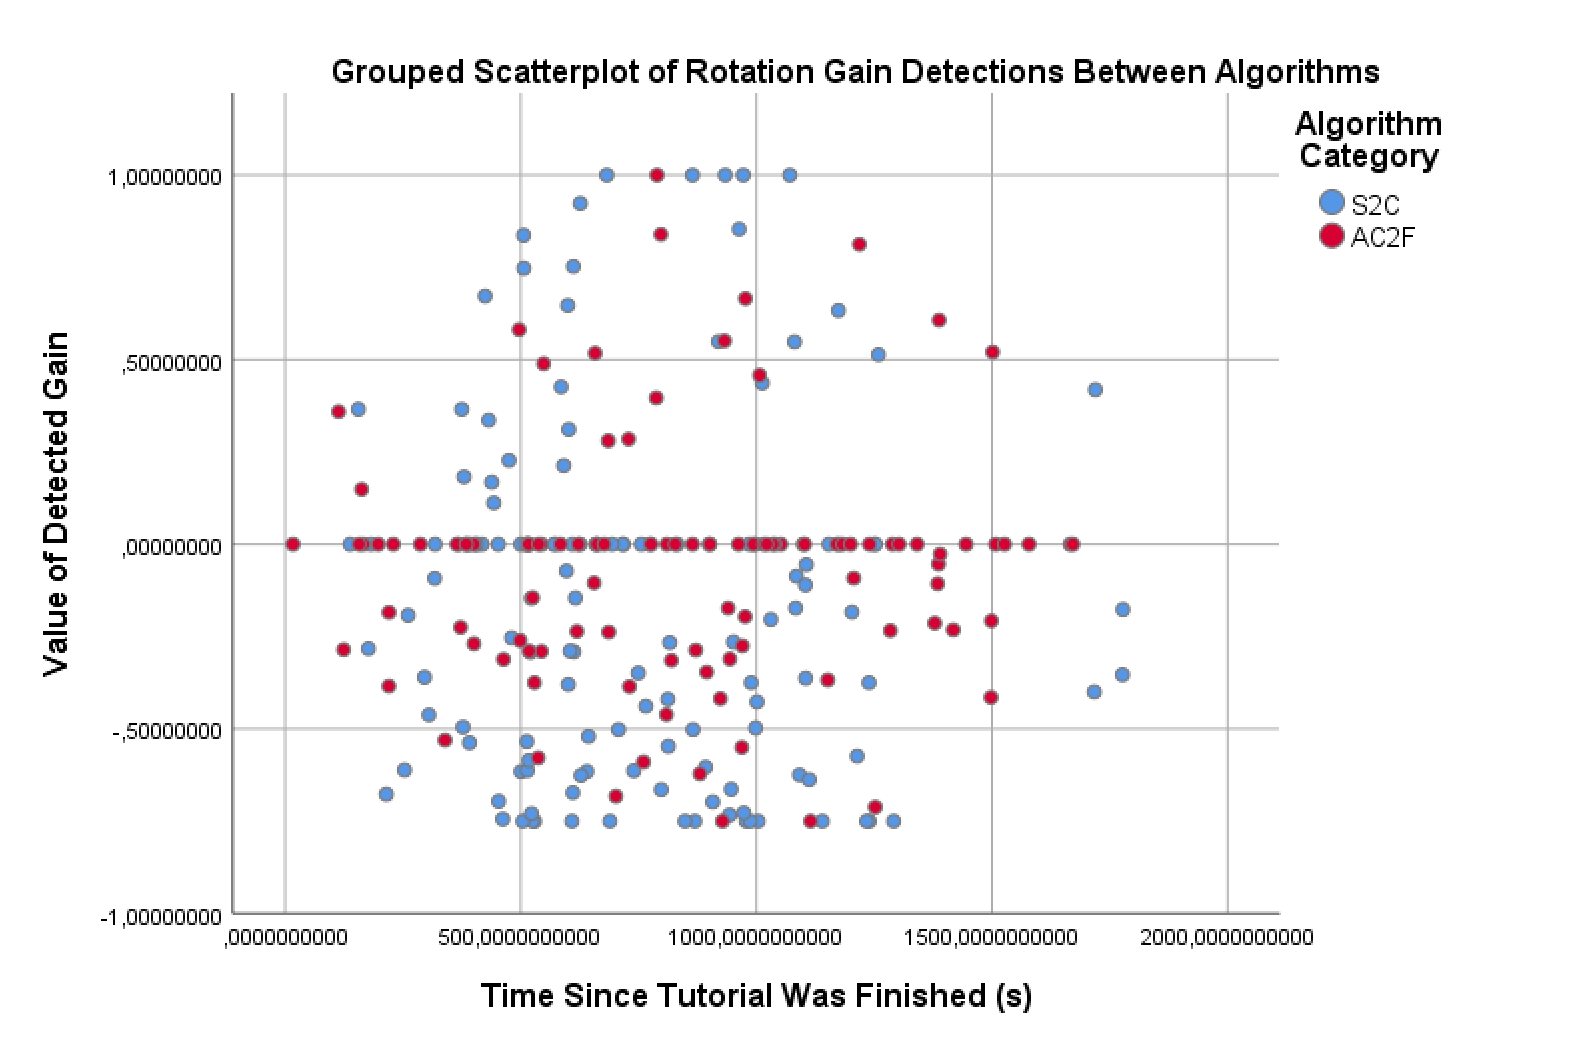
\includegraphics[width=0.75\textwidth]{figures/graphs/RawRotationDetections.png}
    \caption[Raw Detection Scatterplot For Rotation Gains]{This scatterplot shows the raw data, including outliers for rotation detections between the two employed algorithms. S2C is used for the walking state while AC2F is used for the fighting state.}
    \label{fig:rawRotationDetectionData}
\end{figure}

Before seeing the post-processed sample of rotation gain detections, it might be interesting to first see how the raw data looks like. This raw data can be seen in Figure~\ref{fig:rawRotationDetectionData}. The various cases where detected gains are at a value of 0 is what the post-processing step aimed to minimise. 

\subsubsection{Finalised Rotation Detections Sample}
The post processing step which was mentioned in Section~\ref{sec:ex1postprocessing} resulted in 52 additional rotation gain detection events. This addition results in a total of 213 rotation gain detections throughout the entire sample. The processed data can be seen in Figure~\ref{fig:rotationDetectionDataByAlgorithm}, where it is grouped by algorithm and Figure~\ref{fig:rotationDetectionDataByParticipant}, where it is grouped by participant ID. To provide some additional visualisation, a line chart showing the progression of detections between participants can be seen in Figure~\ref{fig:negativeRotationDetectionLineChart} and Figure~\ref{fig:positiveRotationDetectionLineChart}.

 A figure illustrating the incremental progression of rotation gains over time for participant 16 (the author) can be seen in Figure~\ref{fig:authorRotationProgression}. Finally, individual scatterplots for negative/positive rotation gain detections with an included regression line can be found in Figure~\ref{fig:negRotRegLine} and Figure~\ref{fig:posRotRegLine}. It should be noted that some participants are not shown in these graphs as they did not provide any detection events. 

\begin{figure}[tbph]
    \centering
    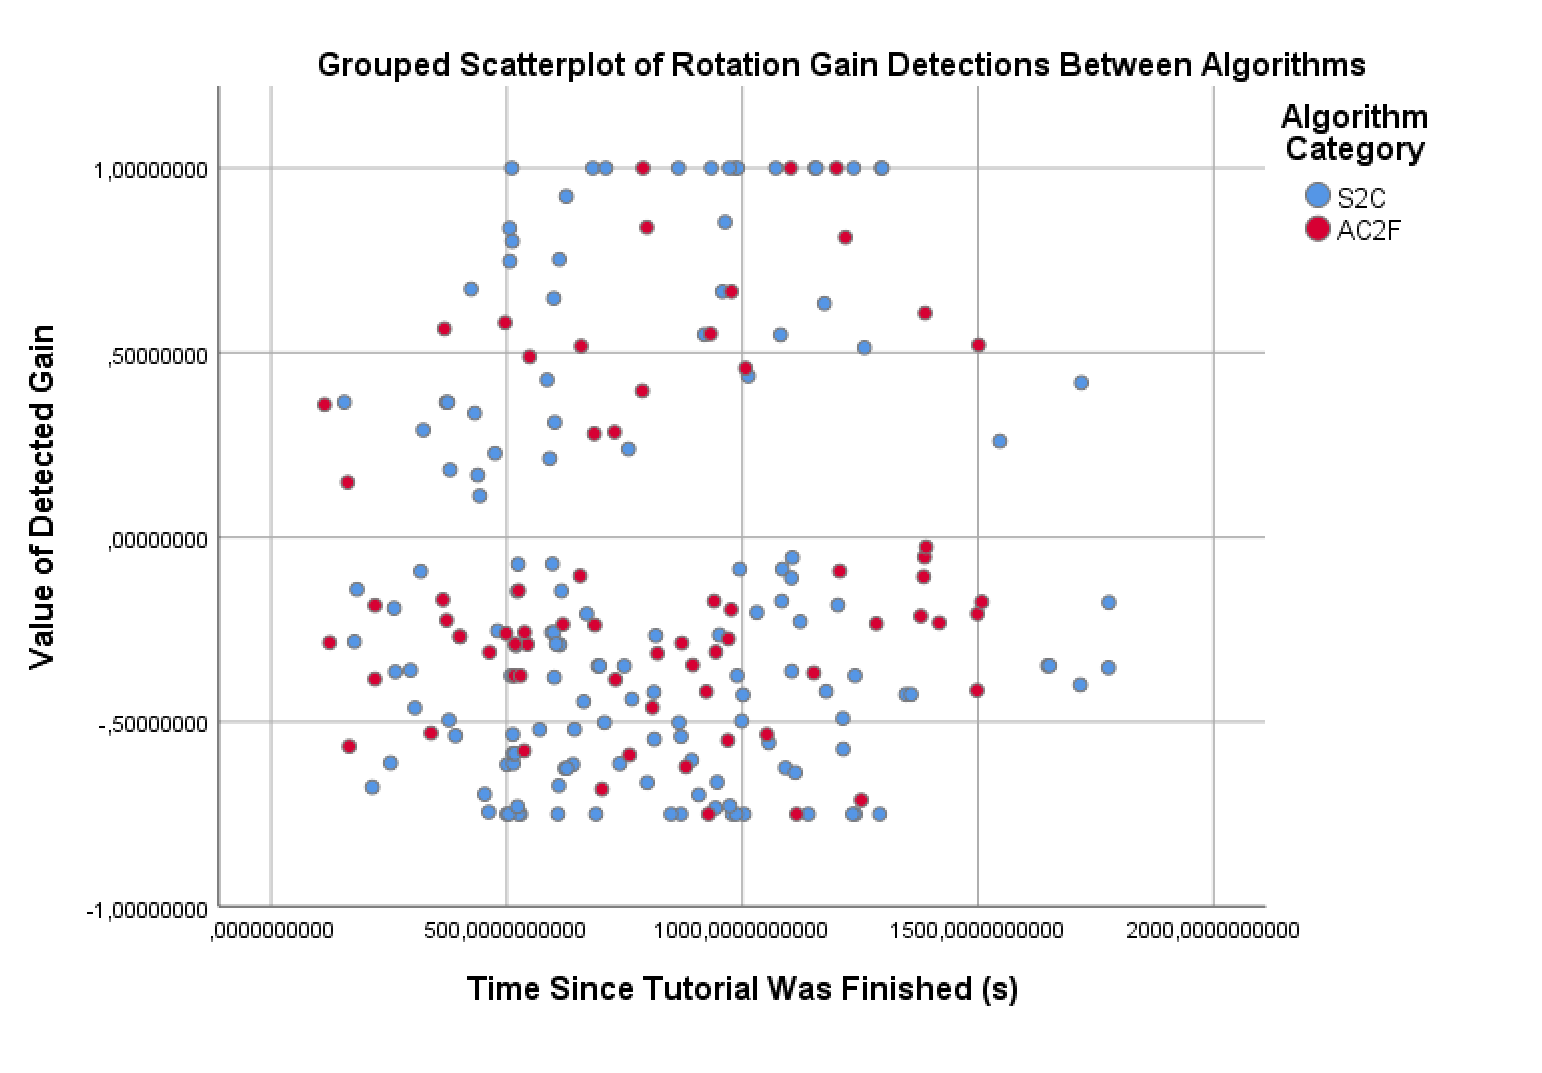
\includegraphics[width=0.75\textwidth]{figures/graphs/ProcessedRotationDetections.png}
    \caption[Finalised Detection Scatterplot For Rotation Gains, Grouped by Algorithm]{This scatterplot shows the finalised data of rotation gain detections and is grouped by algorithm.}
    \label{fig:rotationDetectionDataByAlgorithm}
\end{figure}

\begin{figure}[tbph]
    \centering
    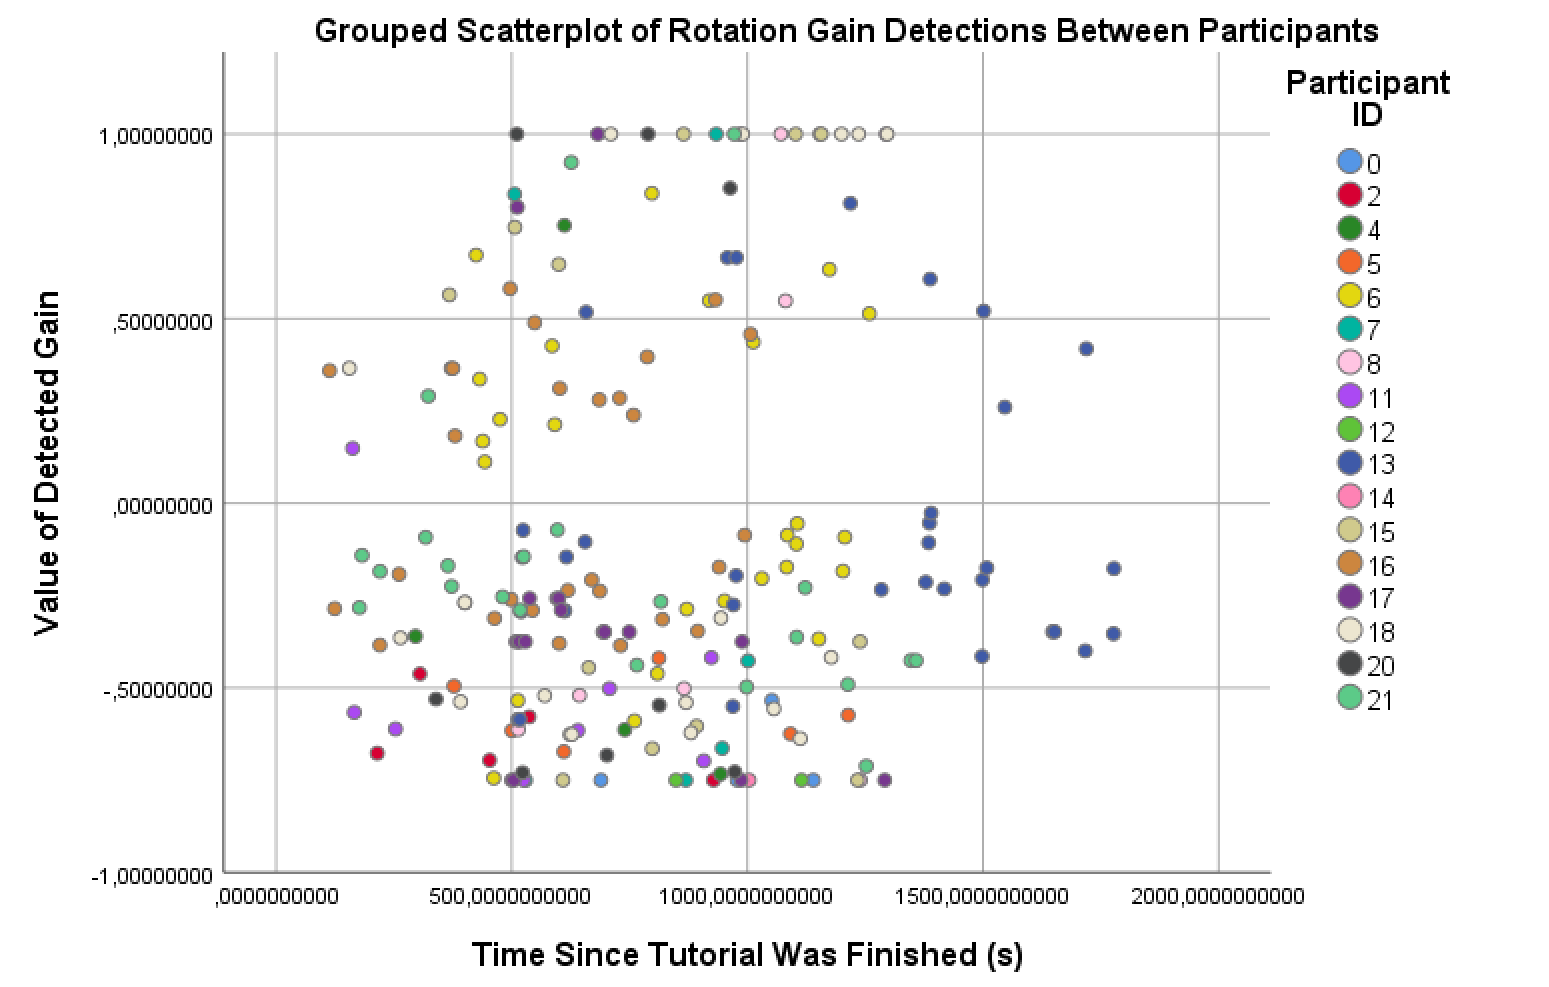
\includegraphics[width=0.75\textwidth]{figures/graphs/ProcessedRotationDetectionsByParticipant.png}
    \caption[Finalised Detection Scatterplot For Rotation Gains, Grouped by Participant ID]{This scatterplot shows the finalised data of rotation gain detections and is grouped by participant ID. Some ID's are not present as these participants did not notice any redirection or misunderstood the task they were given.}
    \label{fig:rotationDetectionDataByParticipant}
\end{figure}

\begin{figure}[tbph]
    \centering
    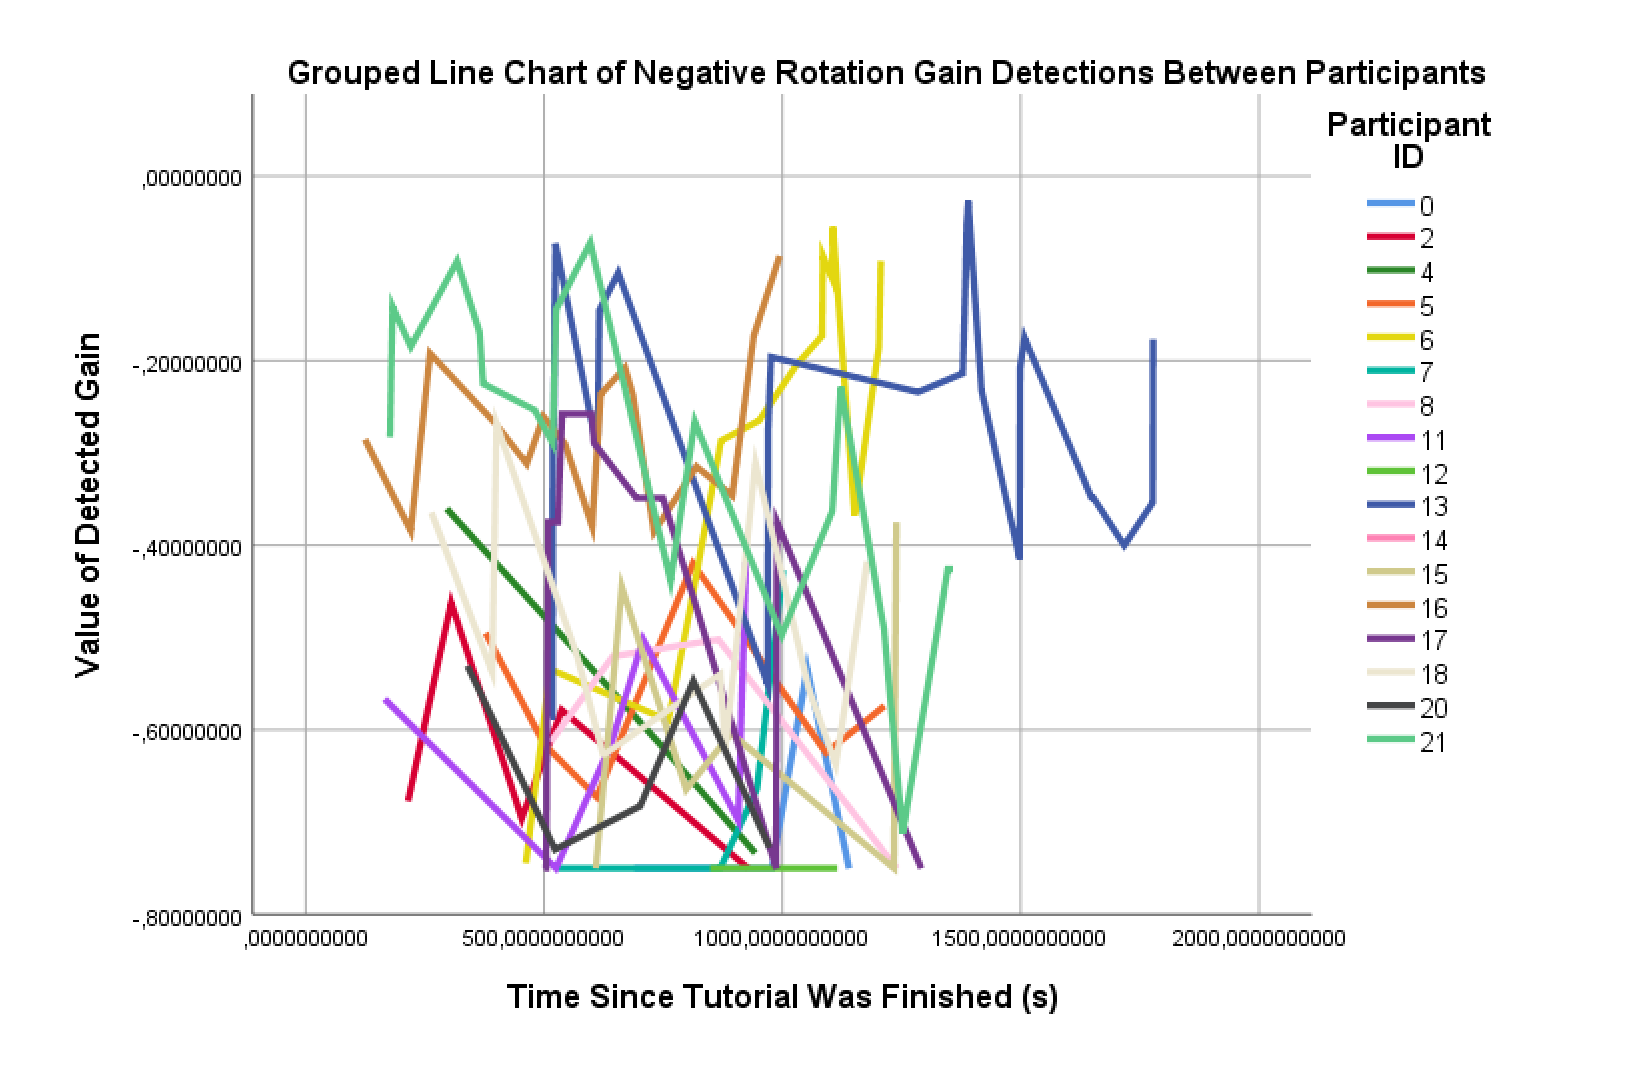
\includegraphics[width=0.75\textwidth]{figures/graphs/NegativeRotationDetectionsLineChart.png}
    \caption[Line Chart of Negative Rotation Gain Detections Between Participants]{This line chart shows the progression in negative rotation gain detections between participants.}
    \label{fig:negativeRotationDetectionLineChart}
\end{figure}

\begin{figure}[tbph]
    \centering
    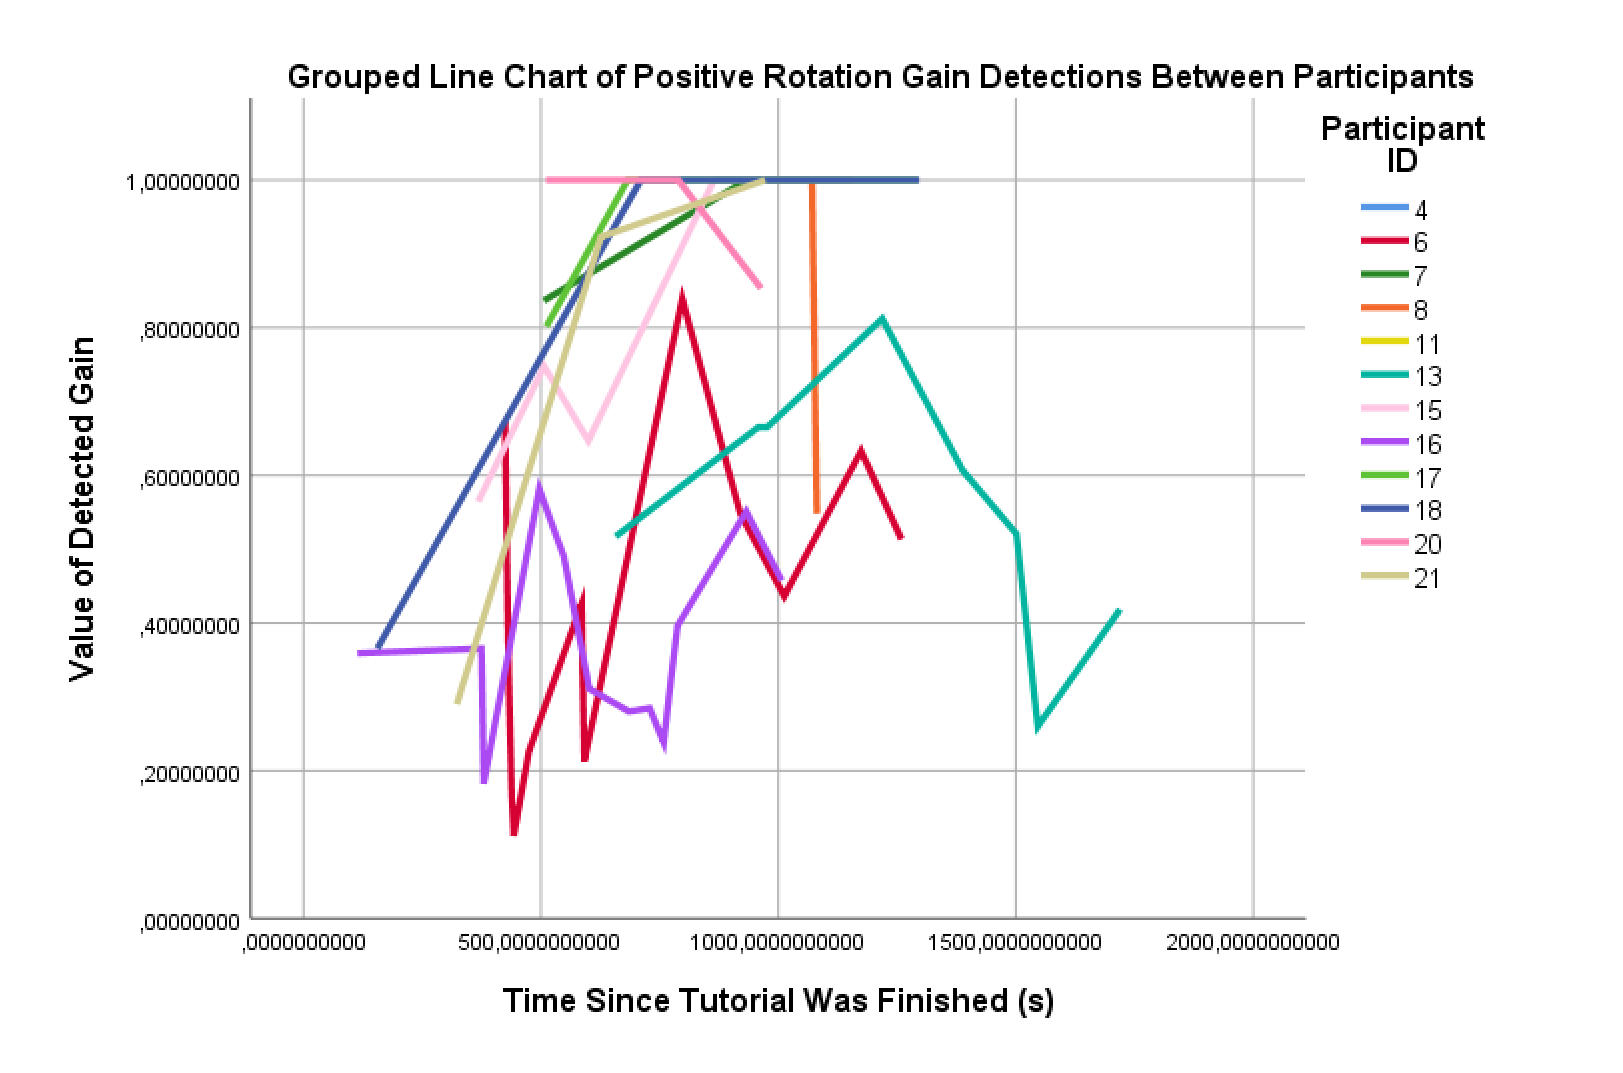
\includegraphics[width=0.75\textwidth]{figures/graphs/PositiveRotationDetectionsLineChart.png}
    \caption[Line Chart of Positive Rotation Gain Detections Between Participants]{This line chart shows the progression in positive rotation gain detections between participants.}
    \label{fig:positiveRotationDetectionLineChart}
\end{figure}

\begin{figure}[tbph]
    \centering
    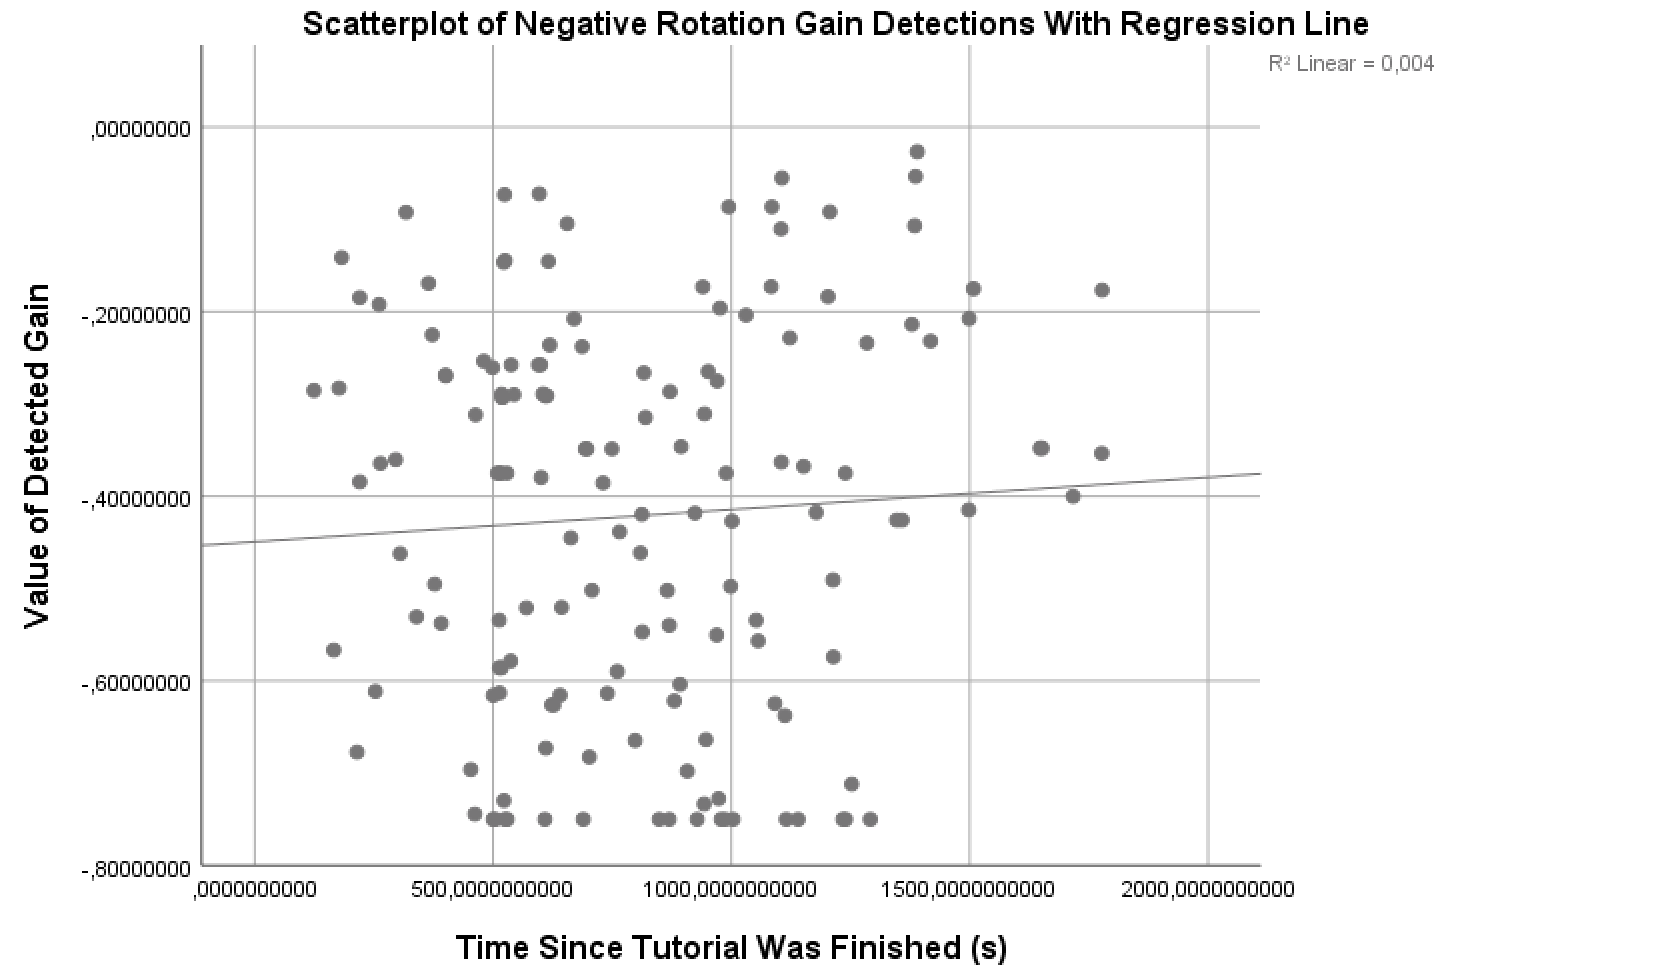
\includegraphics[width=0.75\textwidth]{figures/graphs/NegRotDetectionsRegLine.png}
    \caption[Scatterplot For Negative Rotation Gain Detections Including Regression Line]{This scatterplot shows the spread of negative rotation gain detections with an included regression line.}
    \label{fig:negRotRegLine}
\end{figure}

\begin{figure}[tbph]
    \centering
    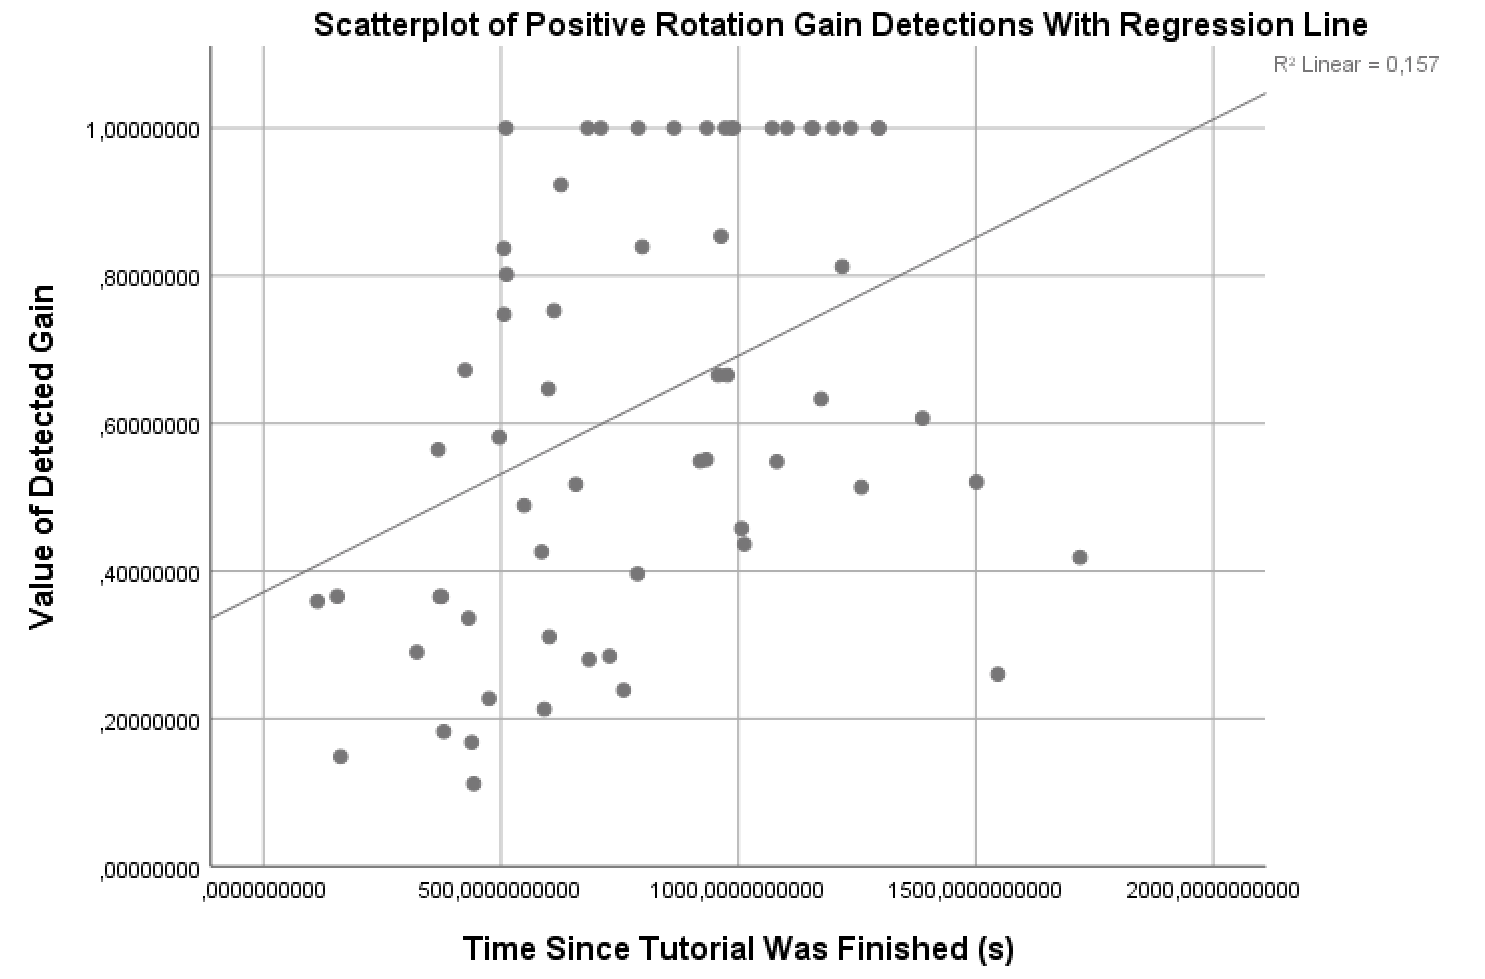
\includegraphics[width=0.75\textwidth]{figures/graphs/PosRotDetectionsRegLine.png}
    \caption[Scatterplot For Positive  Rotation Gain Detections Including Regression Line]{This scatterplot shows the spread of positive rotation gain detections with an included regression line.}
    \label{fig:posRotRegLine}
\end{figure}

\begin{figure}[tbph]
    \centering
    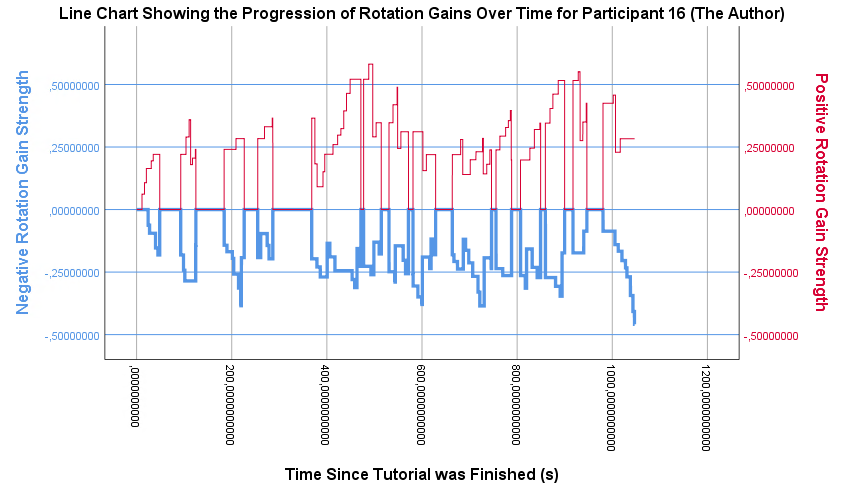
\includegraphics[width=0.75\textwidth]{figures/graphs/rotationGainProgressionAuthor.png}
    \caption[Line Chart Showing the Progression of Rotation Gains for Participant 16]{This line chart shows the progression of rotation gains over time for participant 16. Rotation gains gradually increase over time until they are detected, after which they are dropped by 50\%. Sections of time where gains are 0 are during distractor battles where the future virtual path has been aligned with the physical room centre.}
    \label{fig:authorRotationProgression}
\end{figure}

\subsection{Curvature Detections}
\begin{figure}[tbph]
    \centering
    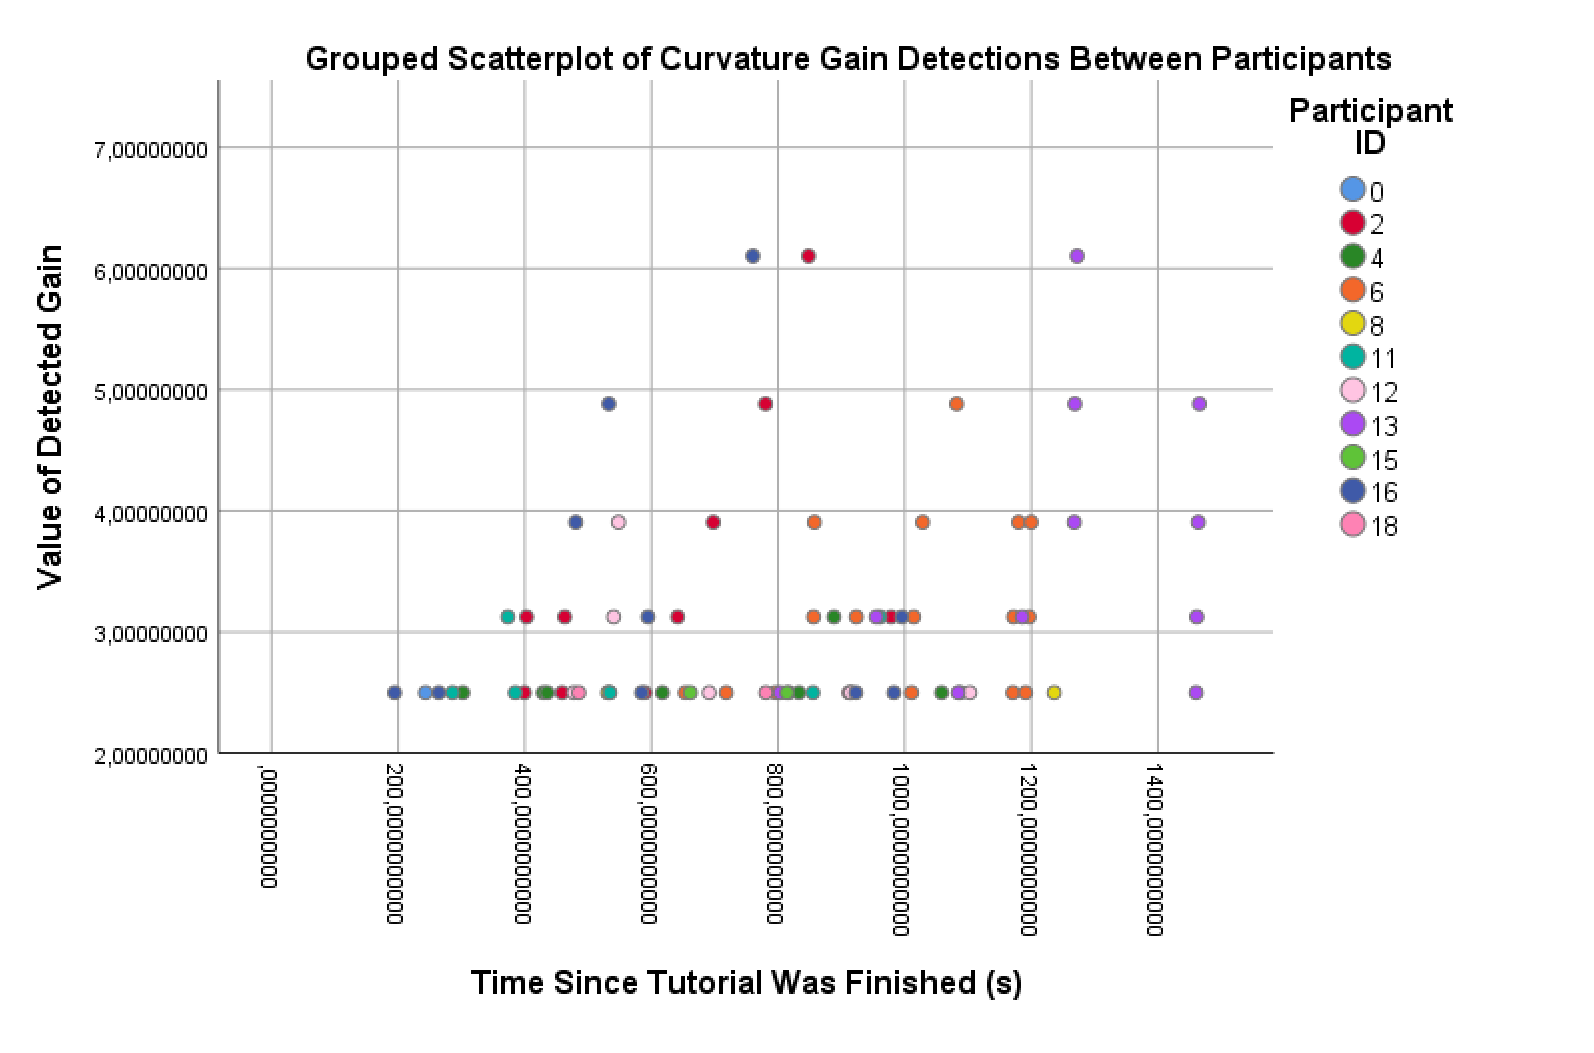
\includegraphics[width=0.75\textwidth]{figures/graphs/CurvatureDetectionScatter.png}
    \caption[Finalised Detection Scatterplot For Curvature Gains, Grouped by Participant ID]{This scatterplot shows the finalised data of curvature gain detections and is grouped by participant ID. Curvature values in this case are defined as the radius of the curvature arc.}
    \label{fig:curvatureDetectionData}
\end{figure}

The various curvature gain detection events that happened during the walking phase of Ensemble Retriever can be seen in Figure~\ref{fig:curvatureDetectionData}.

\subsection{Mean Detection Thresholds}
\begin{table}[!h]
\centering
\begin{tabularx}{\textwidth}{|X|S|X|}
\hline
\textbf{Type of Gain} & \textbf{Mean Detection Threshold} & \textbf{N (Total Number of Detections)} \\
\hline
\hline
S2C: Positive Rotation Gain & 0.6479 & N = 43 \\
\hline
S2C: Negative Rotation Gain & -0.4631 & N = 101 \\
\hline
AC2F: Positive Rotation Gain & 0.5828 & N = 19 \\
\hline
AC2F: Negative Rotation Gain & -0.3365 & N = 50 \\
\hline
S2C+AC2F: Positive Rotation Gain & 0.6279 & N = 43+19 \\
\hline
S2C+AC2F: Negative Rotation Gain & -0.4212 & N = 101+50 \\
\hline
S2C: Curvature Radius & 3.0978m & N = 78 \\
\hline
\end{tabularx}
\caption[Experiment 1: Mean Detection Thresholds]{This table shows the various detection thresholds that were calculated as the mean of all detection events in each respective category.}
\label{table:ex1DetectionThresholds}
\end{table}

The aggregated mean detection thresholds which have been generated out of the previously presented data can be seen in Table~\ref{table:ex1DetectionThresholds}. 

\subsection{Test for Normality and Choice of Significance Test}
Before performing any statistical significance tests on the data, it is first necessary to test the normality of it. For this, the Shapiro-Wilk~\cite{shapiroWilk} test was used on positive and negative rotation gain detections. There is no possibility to compare different conditions for curvature gains, and as such, no normality test was performed on this data. 

\subsubsection{Positive Rotation Gain Detection Normality}
The Shapiro-Wilk test resulted in $p < 0.001$ for the S2C category and $p = 0.295$ for the AC2F counterpart. The S2C category is thus not normally distributed while AC2F is. 

\subsubsection{Negative Rotation Gain Detection Normality}
The Shapiro-Wilk test resulted in $p < 0.001$ for the S2C category and $p = 0.015$ for AC2F. Both of these are thus not normally distributed.  

\subsubsection{Choice of Significance Test}
Since the data is not normally distributed, it is not possible to use standard tests like the independent samples t-test. Instead, the Mann-Whitney U non-parametric test~\cite{MWUTest} is used as it does not assume normally distributed data. 
   
\subsection{Hypothesis Testing}
Before performing the Mann-Whitney U test, it is first necessary to determine whether the shapes of the data between conditions is similar or not. 
\subsubsection{Mann-Whitney U Shape Test}
\begin{figure}[tbph]
    \centering
    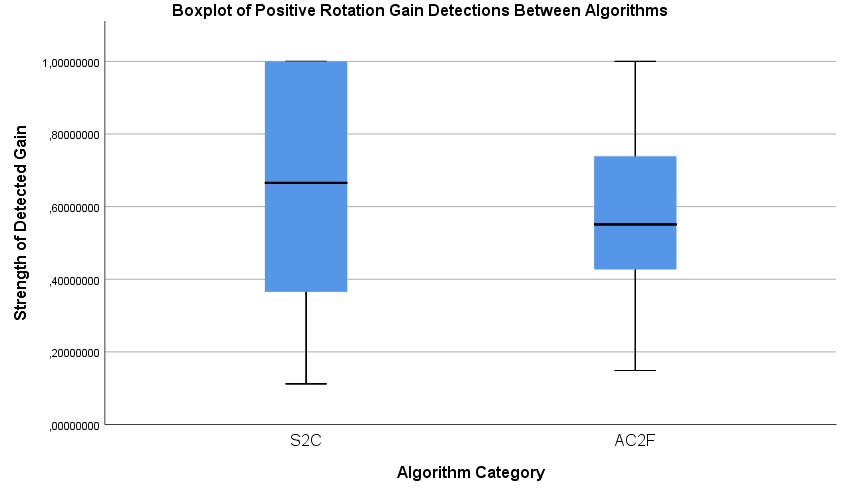
\includegraphics[width=0.75\textwidth]{figures/graphs/PosRotationDetectionBoxplot.png}
    \caption[Boxplot on Positive Rotation Detections in Experiment 1]{This boxplot shows the spread of detected gains between algorithms for positive rotation gains in Experiment 1.}
    \label{fig:posRotEx1Boxplot}
\end{figure}

\begin{figure}[tbph]
    \centering
    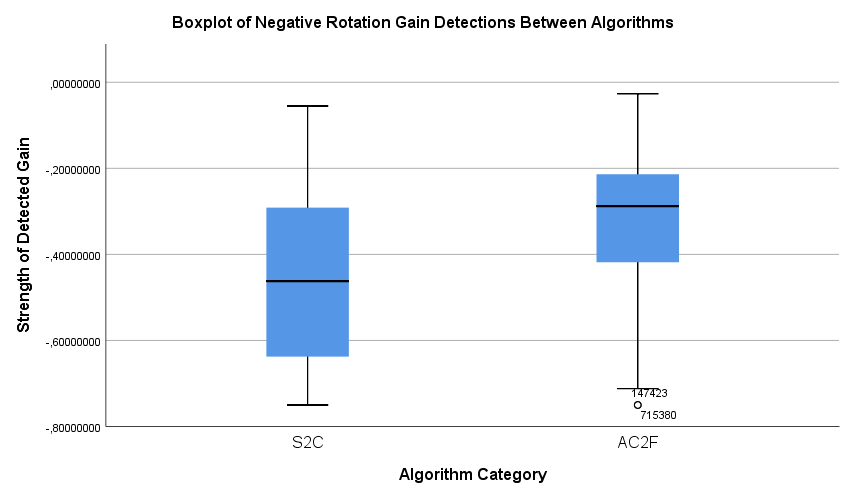
\includegraphics[width=0.75\textwidth]{figures/graphs/NegRotationDetectionBoxplot.png}
    \caption[Boxplot on Negative Rotation Detections in Experiment 1]{This boxplot shows the spread of detected gains between algorithms for negative rotation gains in Experiment 1.}
    \label{fig:negRotEx1Boxplot}
\end{figure}

The shapes of the data can be seen in Figure~\ref{fig:posRotEx1Boxplot} and~\ref{fig:negRotEx1Boxplot}. In general, it does not seem as if the shape between the conditions is similar enough in either of the cases. As such, the Mann-Whitney U comparison will be on mean ranks. It should also be noted that the Mann-Whitney U test's assumption of independent observations cannot be fulfilled due to the within-subjects design of the experiment.

\subsubsection{Mann-Whitney U Results}
The results of the Mann-Whitney U provided a value of $U = 362.5, p = 0.478$ between S2C and AC2F conditions for positive rotation gains. This means that there are no significant differences between the states for these gains. For negative rotation gains, the statistical test resulted in $U = 1639, p < 0.001$, meaning that it is significantly harder to notice negative rotation gains in the walking state in Ensemble Retriever.

\subsection{Demographic Insights}
\begin{figure}[tbph]
    \centering
    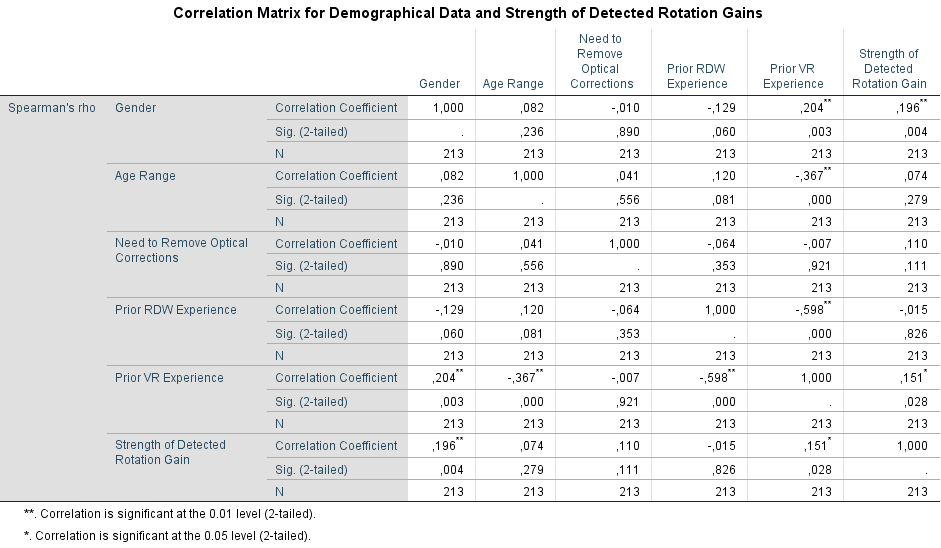
\includegraphics[width=0.8\textwidth]{figures/graphs/DemographicalCorrelationsEx1.png}
    \caption[Experiment 1 Demographic Correlation Matrix]{Correlation matrix for the demographic data in Experiment 1 and the rotation gains that were detected. N values are 213 as there were 213 rotation gain detections.}
    \label{fig:ex1demogcorrelationmatrix}
\end{figure}

In order to look for demographic insights, a correlation analysis has been conducted. This analysis focuses on rotation gain detections and makes use of the Spearman's Rho correlation test as the detection data is not fully normally distributed. The correlation matrix can be seen in Figure~\ref{fig:ex1demogcorrelationmatrix}. The most interesting among these correlations is the positive correlation between prior VR experience and the strength of detected gains. As such, a deeper analysis has been conducted in Section~\ref{sec:ex1demogDiscussion} to gain insights as to why this is the case. 

\subsubsection{Prior VR Experience and Rotation Gain Detections}
\begin{figure}[tbph]
    \centering
    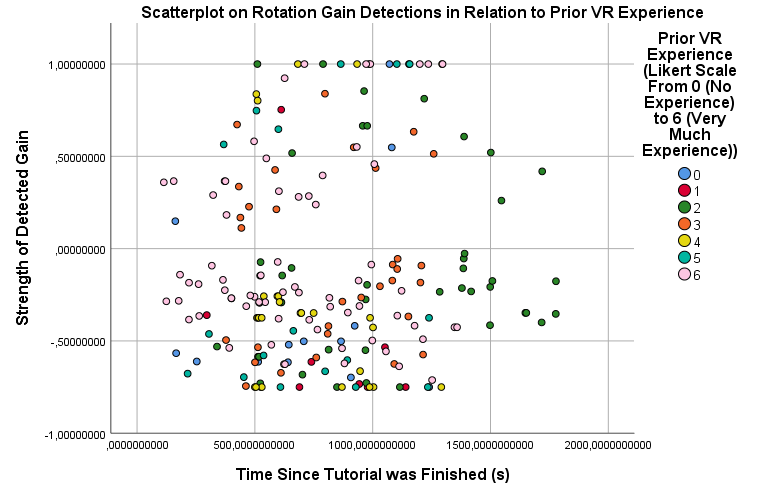
\includegraphics[width=0.75\textwidth]{figures/graphs/PriorVRExperienceDetectionScatter.png}
    \caption[Scatterplot on Rotation Gain Detections in Relation to Prior VR Experience]{This scatterplot shows the rotation gains that were detected in Experiment 1 and their relation to prior VR experience.}
    \label{fig:rotationGainDetectionScatterVRExperience}
\end{figure}

\begin{figure}[tbph]
    \centering
    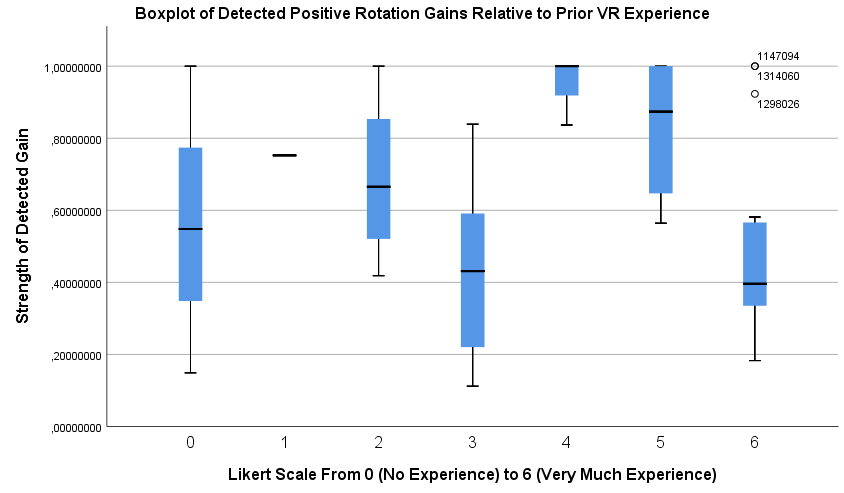
\includegraphics[width=0.75\textwidth]{figures/graphs/PosRotDetectionsByVRExperience.png}
    \caption[Boxplot on Detected Positive Rotation Gains by VR Experience]{This boxplot shows the spread of detected positive rotation gains in relation to prior VR experience.}
    \label{fig:posRotDetectionBoxplotVRExperience}
\end{figure}

\begin{figure}[tbph]
    \centering
    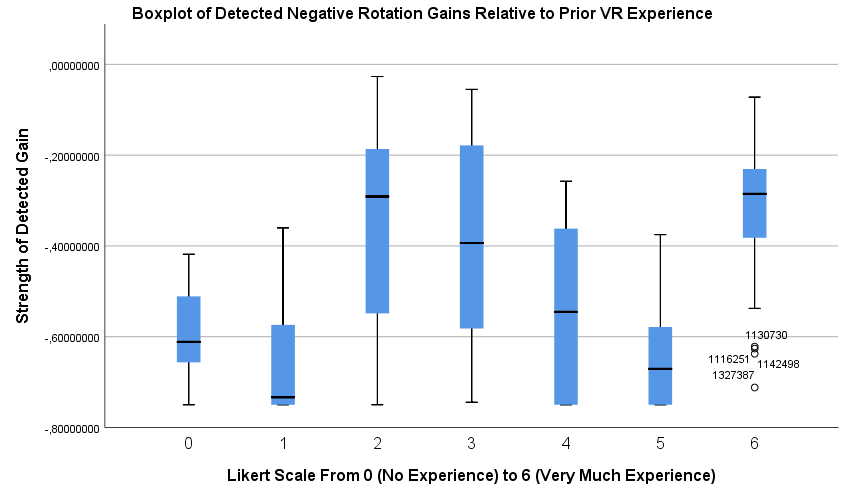
\includegraphics[width=0.75\textwidth]{figures/graphs/NegRotDetectionsByVRExperience.png}
    \caption[Boxplot on Detected Negative Rotation Gains by VR Experience]{This boxplot shows the spread of detected negative rotation gains in relation to prior VR experience.}
    \label{fig:negRotDetectionBoxplotVRExperience}
\end{figure}

As a basis for the later discussion, a scatterplot on the strength of rotation gain detections in relation to prior VR experience can be seen in Figure~\ref{fig:rotationGainDetectionScatterVRExperience}. Boxplots for positive and negative gains can be seen in Figure~\ref{fig:posRotDetectionBoxplotVRExperience} and~\ref{fig:negRotDetectionBoxplotVRExperience}.


\subsubsection{Qualitative Feedback}
The participants also provided some written qualitative feedback through the post-test questionnaire. This section summarises the feedback that was provided on a question by question basis. 

\paragraph{Whether the Participants Found Any Bugs or Glitches}
Some participants experienced minor controller tracking problems when standing in certain areas of the physical tracking space. These were quickly resolved by holding their controllers up in the air. 

\paragraph{Whether the Participants Found the Experience Enjoyable}
In general, participants found the experience to be very positive. Despite this, some mentioned that the experience was rather long, so fighting the same distractors repeatedly got a bit annoying towards the end.

\paragraph{How the Participants Felt About the Redirection Techniques}
When noticed, participants mentioned that the redirection felt rather odd initially. After a while, some participants got used to the effect and found it to be effective while others mentioned it was a bit awkward and annoying. 

\paragraph{Whether the Participants Had Any Problems Throughout Their Experience}
In general, participants mentioned that it was rather frustrating to untangle themselves from the HMD cable as they played. Three participants also mentioned that they experienced a mild amount of discomfort due to the redirection, but that they did not feel like it was enough to mention during the experiment. 

\paragraph{Additional Comments From Participants}
Other than the already mentioned feedback, participants did provide some additional comments on how they felt the experience could be improved. The majority of this feedback has been kept in mind when making changes for Experiment 2. In particular, participants wanted some of the distractors to fire slightly faster projectiles as some of the slower ones became a bit boring over time. The full list of software changes between Experiment 1 and 2 can be seen in Section~\ref{sec:changesBetweenExperiments}.

\subsection{Summary}
\begin{table}[h!]
\centering
\scalebox{0.9}{
\begin{tabularx}{\textwidth}{|X|X|}
\hline
Variable & Context \\
\hline
Size + Shape of Physical Tracking Space & 5m x 5.75m rectangle \\
\hline
Optical Flow/Visual Density in VE & Low Poly Artstyle. Limited visual density outside of environmental trees and shining mushrooms. The walkable environment is fully open. The player has to fight enemy distractors while exploring which move around the player and shoot various salient projectiles that might contribute to increased optical flow and visual density. See figures in Chapter~\ref{chap:implementation} for examples.\\
\hline
Hardware: HMD Field of View & HTC Vive. ~145 diagonal degrees FoV. \\
\hline
Speed of Walking & \textasciitilde$0.2576$ $m/s$ on average (Total distance travelled / Total time spent walking between participants). Static curvature gains employed. \\
\hline
Engagement/Distraction & The participants played through a VR game which consisted of walking around, collecting clues (working memory task) and fighting enemy distractors while exploring. Overall engagement levels based on feedback and observation of participants could be considered as high. \\
\hline
Awareness of Redirection & Participants were informed of redirection and the basics of redirected walking. The concept of distractors was not directly explained, but mentioned in the information/consent sheet. \\
\hline
Gender & 20M, 2F (One among the 22 participants was excluded from the data analysis)\\
\hline
Estimation Method & Incrementally and randomly increasing one gain at random timesteps. Rotation gain is halved when detected, curvature radius is multiplied by 25\% when detected. \\
\hline
Adaptation: Curvature Gains & The experiment employed an incremental gains method for estimation. Gains would as such, gradually increase over time. Some adaptation could be possible, but the curvature detection data cannot answer this. \\
\hline
Adaptation: Positive Rotation Gains & The data does appear to point towards a potential adaptation towards positive rotation gains. The variability of negative rotation gain detections makes it hard to say whether this also is true for these. \\
\hline
Prior VR Experience & While relatively hard to directly conclude with the current data sample, participants with the highest amount of VR experience were the most sensitive towards redirection. Those with no prior VR experience were among the least sensitive. It should also be noted that some participants who had no prior VR experience could not detect any redirection as well. \\
\hline
\end{tabularx}}
\caption[Experiment 1: Summary Over Contextual Variables in Relation To Detection Thresholds]{Summary of variables from Chapter~\ref{chap:relatedWork} with some additions and how Experiment 1 relates to these.}
\label{table:ex1VariableSummary}
\end{table}

A contextual summary of how the various variables from Chapter~\ref{chap:relatedWork} relate to this experiment can be found in Table~\ref{table:ex1VariableSummary}. It also includes some potentially new and relevant variables based on the results that have been shown. In general, the results showed that negative rotation gains are significantly easier to detect during battles (Mann-Whitney U: $U = 1639, p < 0.001$), compared to when walking around. No significant difference could be found for positive rotation gains between the walking and battle states (Mann-Whitney U: $U = 362.5, p = 0.478$). 